\documentclass[tikz]{standalone}

\usepackage[T1]{fontenc}
\usepackage[utf8]{inputenc}
\usepackage{eulervm}
\usepackage{amsmath}
\usepackage{bm}
\usepackage{tikz}
\usepackage{environ}

\usetikzlibrary{fit}
\usetikzlibrary{patterns}
\usetikzlibrary{arrows}

\usepackage{color}

\definecolor{Comment}{RGB}{97,161,176}

\definecolor{btfGreen}{RGB}{51,160,44}
\definecolor{btfRed}{RGB}{190,60,90}

\definecolor{bleuUni}{RGB}{0, 157, 224}
\definecolor{marronUni}{RGB}{68, 58, 49}
\definecolor{grayMarronUni}{RGB}{60, 60, 60}
\definecolor{grayBleuUni}{RGB}{118, 118, 118}

\definecolor{bluecite}{HTML}{009DE0}

\definecolor{Paired-2}{RGB}{166,206,227}
\definecolor{Paired-1}{RGB}{31,120,180}
\definecolor{Paired-4}{RGB}{178,223,138}
\definecolor{Paired-3}{RGB}{51,160,44}
\definecolor{Paired-6}{RGB}{251,154,153}
\definecolor{Paired-5}{RGB}{227,26,28}
\definecolor{Paired-8}{RGB}{253,191,111}
\definecolor{Paired-7}{RGB}{255,127,0}
\definecolor{Paired-10}{RGB}{202,178,214}
\definecolor{Paired-9}{RGB}{106,61,154}
\definecolor{Paired-12}{RGB}{255,255,153}
\definecolor{Paired-11}{RGB}{177,89,40}
\definecolor{Accent-1}{RGB}{127,201,127}
\definecolor{Accent-2}{RGB}{190,174,212}
\definecolor{Accent-3}{RGB}{253,192,134}
\definecolor{Accent-4}{RGB}{255,255,153}
\definecolor{Accent-5}{RGB}{56,108,176}
\definecolor{Accent-6}{RGB}{240,2,127}
\definecolor{Accent-7}{RGB}{191,91,23}
\definecolor{Accent-8}{RGB}{102,102,102}
\definecolor{Spectral-1}{RGB}{158,1,66}
\definecolor{Spectral-2}{RGB}{213,62,79}
\definecolor{Spectral-3}{RGB}{244,109,67}
\definecolor{Spectral-4}{RGB}{253,174,97}
\definecolor{Spectral-5}{RGB}{254,224,139}
\definecolor{Spectral-6}{RGB}{255,255,191}
\definecolor{Spectral-7}{RGB}{230,245,152}
\definecolor{Spectral-8}{RGB}{171,221,164}
\definecolor{Spectral-9}{RGB}{102,194,165}
\definecolor{Spectral-10}{RGB}{50,136,189}
\definecolor{Spectral-11}{RGB}{94,79,162}
\definecolor{Set1-1}{RGB}{228,26,28}
\definecolor{Set1-2}{RGB}{55,126,184}
\definecolor{Set1-3}{RGB}{77,175,74}
\definecolor{Set1-4}{RGB}{152,78,163}
\definecolor{Set1-5}{RGB}{255,127,0}
\definecolor{Set1-6}{RGB}{255,255,51}
\definecolor{Set1-7}{RGB}{166,86,40}
\definecolor{Set1-8}{RGB}{247,129,191}
\definecolor{Set1-9}{RGB}{153,153,153}
\definecolor{Set2-1}{RGB}{102,194,165}
\definecolor{Set2-2}{RGB}{252,141,98}
\definecolor{Set2-3}{RGB}{141,160,203}
\definecolor{Set2-4}{RGB}{231,138,195}
\definecolor{Set2-5}{RGB}{166,216,84}
\definecolor{Set2-6}{RGB}{255,217,47}
\definecolor{Set2-7}{RGB}{229,196,148}
\definecolor{Set2-8}{RGB}{179,179,179}
\definecolor{Dark2-1}{RGB}{27,158,119}
\definecolor{Dark2-2}{RGB}{217,95,2}
\definecolor{Dark2-3}{RGB}{117,112,179}
\definecolor{Dark2-4}{RGB}{231,41,138}
\definecolor{Dark2-5}{RGB}{102,166,30}
\definecolor{Dark2-6}{RGB}{230,171,2}
\definecolor{Dark2-7}{RGB}{166,118,29}
\definecolor{Dark2-8}{RGB}{102,102,102}
\definecolor{Reds-1}{RGB}{255,245,240}
\definecolor{Reds-2}{RGB}{254,224,210}
\definecolor{Reds-3}{RGB}{252,187,161}
\definecolor{Reds-4}{RGB}{252,146,114}
\definecolor{Reds-5}{RGB}{251,106,74}
\definecolor{Reds-6}{RGB}{239,59,44}
\definecolor{Reds-7}{RGB}{203,24,29}
\definecolor{Reds-8}{RGB}{165,15,21}
\definecolor{Reds-9}{RGB}{103,0,13}
\definecolor{Greens-1}{RGB}{247,252,245}
\definecolor{Greens-2}{RGB}{229,245,224}
\definecolor{Greens-3}{RGB}{199,233,192}
\definecolor{Greens-4}{RGB}{161,217,155}
\definecolor{Greens-5}{RGB}{116,196,118}
\definecolor{Greens-6}{RGB}{65,171,93}
\definecolor{Greens-7}{RGB}{35,139,69}
\definecolor{Greens-8}{RGB}{0,109,44}
\definecolor{Greens-9}{RGB}{0,68,27}
\definecolor{Blues-1}{RGB}{247,251,255}
\definecolor{Blues-2}{RGB}{222,235,247}
\definecolor{Blues-3}{RGB}{198,219,239}
\definecolor{Blues-4}{RGB}{158,202,225}
\definecolor{Blues-5}{RGB}{107,174,214}
\definecolor{Blues-6}{RGB}{66,146,198}
\definecolor{Blues-7}{RGB}{33,113,181}
\definecolor{Blues-8}{RGB}{8,81,156}
\definecolor{Blues-9}{RGB}{8,48,107}


\begin{document}
  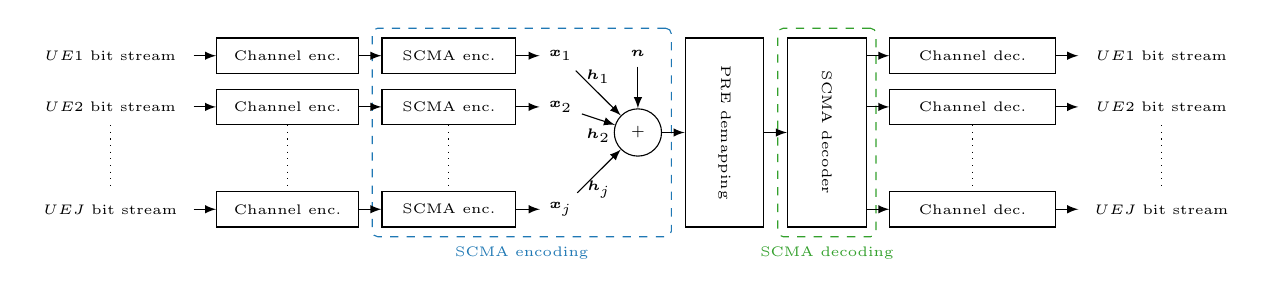
\begin{tikzpicture}[baseline]
    \node[minimum width=2.1cm, minimum height=0.45cm, align=center] (in_bs_uej) at (0.0, 0.225+0.000+0.0) {\tiny{$UEJ$ bit stream}};
    % \node[minimum width=2.1cm, minimum height=0.45cm, align=center] (in_bs_uex) at (0.0, 0.225+0.450+0.2) {\tiny{$UEX$ bit stream}};
    \node[minimum width=2.1cm, minimum height=0.45cm, align=center] (in_bs_ue2) at (0.0, 0.225+0.900+0.4) {\tiny{$UE2$ bit stream}};
    \node[minimum width=2.1cm, minimum height=0.45cm, align=center] (in_bs_ue1) at (0.0, 0.225+1.350+0.6) {\tiny{$UE1$ bit stream}};

    \node[draw=black, minimum width=1.8cm, minimum height=0.45cm, align=center] (cc_uej) at (1.95+0.3, 0.225+0.000+0.0) {\tiny{Channel enc.}};
    % \node[draw=black, minimum width=1.8cm, minimum height=0.45cm, align=center] (cc_uex) at (1.95+0.3, 0.225+0.450+0.2) {\tiny{Channel enc.}};
    \node[draw=black, minimum width=1.8cm, minimum height=0.45cm, align=center] (cc_ue2) at (1.95+0.3, 0.225+0.900+0.4) {\tiny{Channel enc.}};
    \node[draw=black, minimum width=1.8cm, minimum height=0.45cm, align=center] (cc_ue1) at (1.95+0.3, 0.225+1.350+0.6) {\tiny{Channel enc.}};

    \node[draw=black, minimum width=1.7cm, minimum height=0.45cm, align=center] (scma_uej) at (4.0+0.3, 0.225+0.000+0.0) {\tiny{SCMA enc.}};
    % \node[draw=black, minimum width=1.7cm, minimum height=0.45cm, align=center] (scma_uex) at (4.0+0.3, 0.225+0.450+0.2) {\tiny{SCMA enc.}};
    \node[draw=black, minimum width=1.7cm, minimum height=0.45cm, align=center] (scma_ue2) at (4.0+0.3, 0.225+0.900+0.4) {\tiny{SCMA enc.}};
    \node[draw=black, minimum width=1.7cm, minimum height=0.45cm, align=center] (scma_ue1) at (4.0+0.3, 0.225+1.350+0.6) {\tiny{SCMA enc.}};

    \node[minimum width=0.5cm, align=center] (xj) at (5.420+0.3, 0.225+0.000+0.0) {\tiny{$\bm{x}_j$}};
    % \node[minimum width=0.5cm, align=center] (xx) at (5.420+0.3, 0.225+0.450+0.2) {\tiny{$\bm{x}_x$}};
    \node[minimum width=0.5cm, align=center] (x2) at (5.420+0.3, 0.225+0.900+0.4) {\tiny{$\bm{x}_2$}};
    \node[minimum width=0.5cm, align=center] (x1) at (5.420+0.3, 0.225+1.350+0.6) {\tiny{$\bm{x}_1$}};

    \node[draw=black, circle, align=center, minimum width=0.60cm] (plus) at (6.7, 1.20) {\tiny{$+$}};
    \node[align=center, minimum width=0.60cm] (n0) at (6.7, 2.20) {\tiny{$\bm{n$}}};

    \node[draw=black, align=center, minimum width=1.00cm, minimum height=2.40cm, label={[black, rotate=-90]center:\tiny{PRE demapping}}] (dmap)  at (7.8,     1.20) {\tiny{}};
    \node[draw=black, align=center, minimum width=1.00cm, minimum height=2.40cm, label={[black, rotate=-90]center:\tiny{SCMA decoder}} ] (dscma) at (8.8+0.3, 1.20) {\tiny{}};

    \node[draw=black, minimum width=2.1cm, minimum height=0.45cm, align=center] (cd_uej) at (10.65+0.3, 0.225+0.000+0.0) {\tiny{Channel dec.}};
    % \node[draw=black, minimum width=2.1cm, minimum height=0.45cm, align=center] (cd_uex) at (10.65+0.3, 0.225+0.450+0.2) {\tiny{Channel dec.}};
    \node[draw=black, minimum width=2.1cm, minimum height=0.45cm, align=center] (cd_ue2) at (10.65+0.3, 0.225+0.900+0.4) {\tiny{Channel dec.}};
    \node[draw=black, minimum width=2.1cm, minimum height=0.45cm, align=center] (cd_ue1) at (10.65+0.3, 0.225+1.350+0.6) {\tiny{Channel dec.}};

    \node[minimum width=2.1cm, minimum height=0.45cm, align=center] (out_bs_uej) at (13.05+0.3, 0.225+0.000+0.0) {\tiny{$UEJ$ bit stream}};
    % \node[minimum width=2.1cm, minimum height=0.45cm, align=center] (out_bs_uex) at (13.05+0.3, 0.225+0.450+0.2) {\tiny{$UEX$ bit stream}};
    \node[minimum width=2.1cm, minimum height=0.45cm, align=center] (out_bs_ue2) at (13.05+0.3, 0.225+0.900+0.4) {\tiny{$UE2$ bit stream}};
    \node[minimum width=2.1cm, minimum height=0.45cm, align=center] (out_bs_ue1) at (13.05+0.3, 0.225+1.350+0.6) {\tiny{$UE1$ bit stream}};

    \node[draw=Paired-1, rounded corners=2pt, label={[Paired-1]below:\tiny{SCMA encoding}}, minimum height=2cm, dashed, fit=(scma_uej) (scma_ue1) (plus)] {};
    \node[draw=Paired-3, rounded corners=2pt, label={[Paired-3]below:\tiny{SCMA decoding}}, minimum height=2cm, dashed, fit=(dscma)] {};

    \draw[->,>=latex] (n0) -- (plus);

    \draw[->,>=latex] (in_bs_uej) -- (cc_uej);
    \draw[->,>=latex] (in_bs_ue2) -- (cc_ue2);
    \draw[->,>=latex] (in_bs_ue1) -- (cc_ue1);

    \draw[->,>=latex] (cc_uej) -- (scma_uej);
    \draw[->,>=latex] (cc_ue2) -- (scma_ue2);
    \draw[->,>=latex] (cc_ue1) -- (scma_ue1);

    \draw[->,>=latex] (scma_uej) -- (xj);
    \draw[->,>=latex] (scma_ue2) -- (x2);
    \draw[->,>=latex] (scma_ue1) -- (x1);

    \draw[->,>=latex] (xj) -- (plus) node [midway, below] {\tiny{$\bm{h}_j$}};
    \draw[->,>=latex] (x2) -- (plus) node [midway, below] {\tiny{$\bm{h}_2$}};
    \draw[->,>=latex] (x1) -- (plus) node [midway, above] {\tiny{$\bm{h}_1$}};

    \draw[->,>=latex] (plus) -- (dmap);

    \draw[->,>=latex] (dmap) -- (dscma);

    \draw[->,>=latex] (9.6, 0.225+0.000+0.0) -- (cd_uej);
    \draw[->,>=latex] (9.6, 0.225+0.900+0.4) -- (cd_ue2);
    \draw[->,>=latex] (9.6, 0.225+1.350+0.6) -- (cd_ue1);

    \draw[->,>=latex] (cd_uej) -- (out_bs_uej);
    \draw[->,>=latex] (cd_ue2) -- (out_bs_ue2);
    \draw[->,>=latex] (cd_ue1) -- (out_bs_ue1);

    \draw[dotted] (in_bs_ue2)  -- (in_bs_uej);
    \draw[dotted] (cc_ue2)     -- (cc_uej);
    \draw[dotted] (scma_ue2)   -- (scma_uej);
    \draw[dotted] (cd_ue2)     -- (cd_uej);
    \draw[dotted] (out_bs_ue2) -- (out_bs_uej);
  \end{tikzpicture}
\end{document}